\section[Introduction]{Introduction}
% Første parameter i [] er tekst i header. {} er i indholdsfortegnelsen.

% Slide med emneoverskrift.
\begin{frame}
  \frametitle{}
  \begin{center}
    {\Huge Introduction}
  \end{center}
\end{frame}
\note{
  \begin{itemize}
		\item Notes.
  \end{itemize}
}

% Normal slide:
\begin{frame}
    \frametitle{Introduction}
    %\framesubtitle{Some example subtitle}
    \centering
    \begin{itemize}
      \item Motivation
      \item Problem definition
      \item Methodology
        \begin{itemize}
          \item Feature generation
        \end{itemize}
    \end{itemize}
\end{frame}
\note{
  \begin{itemize}
    \item Say words
  \end{itemize}
}

% Normal slide:
\begin{frame}
    \frametitle{Motivation}
    %\framesubtitle{Some example subtitle}
    \centering
    \begin{itemize}
      \item Internet is used everywhere
      \item Linking is important
        \begin{itemize}
          \item Easier access and navigation
        \end{itemize}
      \item Wikipedia
        \begin{itemize}
           \item Difficult to maintain good link structure
           \item Official guidelines
         \end{itemize}
    \end{itemize}
\end{frame}
\note{
	\begin{itemize}
    \item Notes here...
	\end{itemize}
}

% Normal slide:
\begin{frame}
    \frametitle{Problem definition}
    %\framesubtitle{Some example subtitle}
    \centering
    \begin{itemize}
      \item Different approaches
        \begin{itemize}
          \item Content-based
          \item Structure-based
        \end{itemize}
      \item Often use machine learning
      \item Combination of structure-based and machine learning less commonly used
    \end{itemize}
    \emph{How can a software solution be developed that supports Wikipedia editors by suggesting potential article links using machine learning on a graph structure?}
\end{frame}
\note{
  \begin{itemize}
    \item Notes here...
  \end{itemize}
}

% Normal slide:
\begin{frame}
    \frametitle{Methodology}
    %\framesubtitle{Some example subtitle}
    \begin{columns}[T]
      \begin{column}{0.55\textwidth}
        \begin{itemize}
          \item Data model
          \item Binary classification
          \item Supervised learning
            \begin{itemize}
              \item Featured articles provide labeled training pairs
            \end{itemize}
        \end{itemize}
      \end{column}
      \begin{column}{0.45\textwidth}
        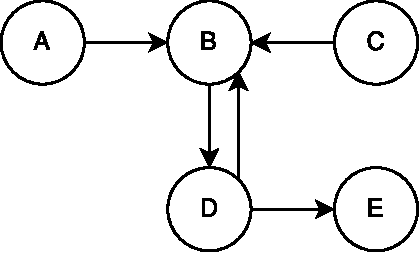
\includegraphics[scale=0.65]{graph}
      \end{column}
    \end{columns}

\end{frame}
\note{
  \begin{itemize}
    \item Notes here...
  \end{itemize}
}

% Normal slide:
\begin{frame}
    \frametitle{Feature generation}
    %\framesubtitle{Some example subtitle}
    \centering
    \begin{itemize}
      \item Need to represent article pairs appropriately
      \item Feature engineering
        \begin{itemize}
          \item Iterative process
          \item Domain knowledge necessary
        \end{itemize}
      \item Feature learning
        \begin{itemize}
          \item More recent approach
          \item Learn the feature representation using machine learning
          \item Less need for domain knowledge
        \end{itemize}
    \end{itemize}
\end{frame}
\note{
  \begin{itemize}
    \item Notes here...
  \end{itemize}
}
